\documentclass[a4paper,11pt]{article}

%\usepackage[ngerman]{babel}         % Neue deutsche Rechtschreibung
\usepackage[T1]{fontenc}            % Bessere Schriftdarstellung
\usepackage{lmodern}                % Aktuelle Schrift

\usepackage[intlimits]{amsmath}     % Zusaetzliche Matheumgebungen
\usepackage{amssymb}                % Mathematische Symbole
\usepackage{graphicx}               % notwendig fuer \includegraphics
\usepackage{fancyhdr}               % Kopf- und Fusszeile
\usepackage{lastpage}               % erzeugt Referez zu der letzten Seite
\usepackage{moreverb}               % verbatimtab Umgeung
\usepackage{tikz}
\usepackage{xcolor}
\usetikzlibrary{decorations.pathmorphing,shapes,decorations.text,decorations,calc,positioning,automata,matrix,arrows}


% Seiteneinstelungen
\setlength\textwidth{165mm}           % Breite
\setlength\textheight{235mm}          % Hoehe
\setlength\headheight{41pt}           % Hoehe der Kopfzeile
\setlength\topmargin{-12mm}           % Abstand oben
\setlength\oddsidemargin{0mm}         % Linker Rand
\setlength\parindent{0pt}             % und ohne Einrueckung
\setlength\parskip{1.7\medskipamount} % Absaetze abgesetzt
\sloppy\pagestyle{fancy}

% Kopf- und Fusszeileeinstellungen
\renewcommand{\headrulewidth}{0.4pt} 	%obere Trennlinie
\fancyfoot[C]{Page:~\thepage~of~\pageref{LastPage}} %Seitennummer
\renewcommand{\footrulewidth}{0.4pt} 	%untere Trennlinie

\newcommand{\R}{\mathbb{R}}                 % reelle Zahlen
\newcommand{\N}{\mathbb{N}}                 % natuerliche Zahlen
\newcommand{\e}{\text{e}}                   % eulersche Zahl
\newcommand{\E}[1]{\cdot10^{#1}}            % x 10^{...}
\newcommand{\qed}{\hspace*{\fill}q.e.d.}    % Beweis fertig
\newcommand{\ON}[1]{{\cal O}(#1)}	          %O-Notation

\newcommand{\todo}[1]{\marginpar{\textcolor{red}{TODO: #1}}}

\fancyhead[R]{Malte Josten, 3066184}
\fancyhead[C]{\large{\bf{<Eins Cooler Titel>}}}
\fancyhead[L]{\textbf{Master Thesis - Expose}\\ Summer 2023}

\usepackage{listings}

% Unteraufgaben (mit Enumeration)
\def\labelenumi{(\arabic{enumi})}
\parindent0mm % keine Absatzeinrückung

\usepackage[utf8]{inputenc}

\usepackage{enumitem}
\setlist{nosep}

\usepackage{dirtree}
\usepackage{booktabs}

\begin{document}
\section{Background}
The goal of this thesis is to design and develop a framework which should enable a smart home user to only specify the desired state of the smart home and do not need to worry about the different "ways to get there".
Therefore, the cognitive load is lowered and the overall experience when using and interacting with smart homes is expected to improve.
In conventional smart home systems, the user instructs the smart home system to, e.g., close the windows and increase the heater's temperature to 24°C.
With the finished framework, it is only necessary to specify the desired outcome, e.g., raise the room temperature to 23°C.
The framework/smart home system then decides which action(s) yield(s) the desired outcome (most efficiently) and controls the smart devices accordingly.


\section{The Framework}
- Read in sensor data and train prediction model in or outside of framework? \\
- Own "Smart Home Interface" and/or connect to existing APIs (if available)? \\
- It should be possible to use an abritary prediction method and integrate all available smart home systems (if API is available) \\
\begin{figure}[h!]
   \centering
   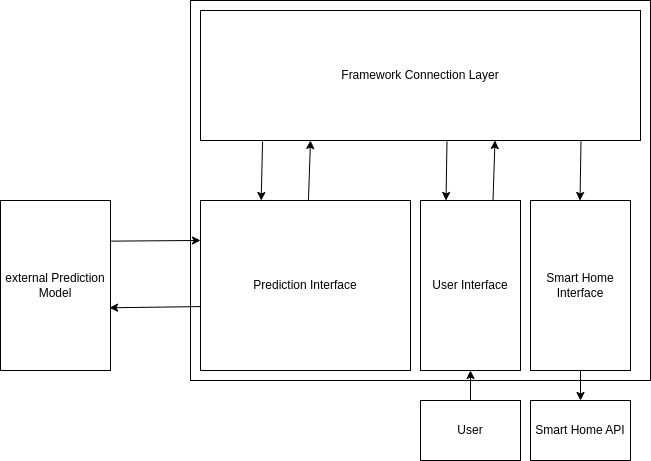
\includegraphics[width=.75\textwidth]{fw-architecture.png} 
   \caption{Sample framework architecture}
\end{figure}
%Reading in the sensor data, training the models and passing forward instructions, e.g., "Give me an efficient control sequence to raise the room's temperature to 24 degrees," should be done entirely be the framework.
%The framework also should offer an interface to one can connect the smart home API to pass forward the acquired control sequence.

\newpage
\section{Proof of Concept}
To show that the developed framework works as intended and a variety of prediction techniques can be integrated, two prediction methods will be implemented, trained, and integrated into the framework.
For this, fitting AI-model and a small program which uses functions derived from symbolic regression will be created.
Both will be trained with a (small) real-world sensor data set.
To give a complete Proof Of Concept, technically it is necessary to also make the connection to at least one smart home system.
Given the situation, this might not be possible and a simulated/artificial smart home system needs to be deployed and integrated accordingly.


\section{Evaluation}
The evaluation will be based on the success of the proof of concept and the framework (architecture) will be assessed regarding the following four aspects:
\begin{itemize}
    \item[1.] Inversion of Control
    \item[2.] Default Behavior
    \item[3.] Extensibility
    \item[4.] Compability
\end{itemize}

\newpage
\subsection{(Example) Structure}
\dirtree{%
    .1 .
    .2 Abstract.
    .2 1 Introduction.
    .2 2 Background.
    .3 2|1 Smart Home Technologies.
    .3 2|2 (Software) Framework Principles.
    .3 2|3 Prediction Techniques.
    .2 3 Previous/Related Work.
    .2 4 Framework.
    .3 4|1 Design/Architecture.
    .3 4|2 Implementation.
    .2 5 Proof Of Concept.
    .3 5|1 Available Data (small set of real world measurements).
    .3 5|2 Artificial Intelligence.
    .4 5|2|1 Network Model.
    .4 5|2|2 Training.
    .3 5|3 Symbolic Regression.
    .4 5|3|1 Used method(s).
    .4 5|3|2 Results.
    .3 (5|4 Validation (with real world data)).
    .2 6 Evaluation.
    .2 7 Conclusion and Future Work.
}

\section{Time Management}
\begin{minipage}[t]{.45\textwidth}
    \textbf{Week 1-2}
    \begin{itemize}
        \item Framework Design
    \end{itemize}
    \textbf{Week 5-6}
    \begin{itemize}
        \item Framework Implementation
    \end{itemize}
    \textbf{Week 9-10}
    \begin{itemize}
        \item PoC: AI
    \end{itemize}
    \textbf{Week 13-14}
    \begin{itemize}
        \item Ch. 4 Framework
    \end{itemize}
    \textbf{Week 17-18}
    \begin{itemize}
        \item Ch. 5 Proof of Concept
        \item[]
        \item[]
    \end{itemize}
    \textbf{Week 21-22}
    \begin{itemize}
        \item Ch. 2 Background
        \item Ch. 3 Related Work
        \item Ch. 1 Introduction
        \item Ch. 7 Conclusion
    \end{itemize}
    \textbf{Week 25-26}
    \begin{itemize}
        \item Buffer
    \end{itemize}
\end{minipage}
\hfill
\begin{minipage}[t]{.45\textwidth}
    \textbf{Week 3-4}
    \begin{itemize}
        \item Framework Design 
    \end{itemize}
    \textbf{Week 7-8}
    \begin{itemize}
        \item Framework Implementation
    \end{itemize}
    \textbf{Week 11-12}
    \begin{itemize}
        \item PoC: Symbolic Regression
    \end{itemize}
    \textbf{Week 15-16}
    \begin{itemize}
        \item Ch. 4 Framework
    \end{itemize}
    \textbf{Week 19-20}
    \begin{itemize}
        \item Ch. 6 Evaluation
        \item Ch. 2 Background
        \item Ch. 3 Related Work
    \end{itemize}
    \textbf{Week 23-24}
    \begin{itemize}
        \item Buffer
    \end{itemize}
\end{minipage}

%Note: Looking for and organizing related work is done concurrently with all the other tasks.

\end{document}
